\chapter{Implementación}
En este capítulo describiremos detalles de la implementación de nuestro modelo de reconocimiento de números en español. Comenzaremos describiendo el proceso de obtención y tratamiento de datos. Finalmente, mostraremos el esquema de nuestra red neuronal.

\section{Datos}
Para las tareas de reconocimiento de voz es importante encontrar un conjunto de datos adecuado, este servirá para alimentar nuestra red neuronal. Proyectos como \textit{VoxForge}\cite{WEBSITE:21} y \textit{Common Voice}\cite{WEBSITE:22} son iniciativas open source que buscan formar un gran corpus de data para distintos idiomas. Sin embargo en el lenguaje español los datos aún están en proceso de recolección. Por lo cual obtener los datos para una tarea específica resulta complicado.
\subsection{Recolección de datos}
Debido al problema anterior fue necesario realizar una propia recolección de datos. Durante este proceso se obtuvo la información de 12 hablantes. Los cuales proporcionaron grabaciones de voz de la pronunciación de los dígitos $0, 1, .. ., 8, 9$. 
\subsubsection{Conjuntos de datos}
Nuestro conjunto de datos consta de un total de 300 audios los cuales fueron dividos en 2 conjuntos:
\begin{itemize}
	\item \textbf{Training}: Este conjunto es usado para entrenar nuestro modelo. Posee 24 muestra de cada número.
	\item \textbf{Test}: Este conjunto es usar para verificar la precisión de modelo. Posee 11 muestras de cada número.
\end{itemize}

La división del conjunto de datos es mostrada en el cuadro 5.1.

\begin{table}[H]
	\centering
	\begin{tabular}{|c|c|}
		\hline
		\rowcolor{Gray}	Training & Test \\ \hline
		240      & 110   \\ \hline
	\end{tabular}
	\caption{División del conjunto de datos}
\end{table}
Debido a las diferencias de entre las voces de entre personas de diferentes sexos fue necesario tener una variedad de hablantes entre mujeres y varones con el objetivo de construir un modelo más robusto. La distribución de hablantes se muestra en cuadro 5.2.


\begin{table}[H]
	\centering
	\begin{tabular}{|c|c|}
		\hline
		\rowcolor{Gray}Mujeres & Varones \\ \hline
		5      & 7   \\ \hline
	\end{tabular}
	\caption{Distribución de hablantes del conjunto de datos por sexo}
\end{table}


La distribución de acuerdo a la cantidad de audios con Voces Femeninas(VF) y Voces Masculinas(VM) se muestran en el cuadro 5.3.

\begin{table}[H]
	\centering
	\begin{tabular}{|c|c|c|c|}
		\hline
		\rowcolor{Gray} 	\multicolumn{4}{|c|}{conjunto de datos}                    \\ \hline
		\multicolumn{2}{|c|}{Training} & \multicolumn{2}{c|}{Test} \\ \hline
		VF              & VM             & VF          & VM           \\ \hline
		90             & 150           & 40          & 70         \\ \hline
	\end{tabular}
	\caption{División del conjunto en base a la cantidad de audios con voces femeninas y masculinas}
\end{table}

\subsection{Tratamiento de los datos}

\subsubsection{Conversión de formato}
Los audios proporcionados por algunos hablantes se encontraban en un formato ogg, el cual tuvo que ser transformado al formato wav para su procesamiento esto debido a que ogg es más formato usado en teléfonos moviles mientras que el formato wav es más estándar. En el Apéndice \ref{converter} podemos observar el código usado.

\subsection{Obtención de coeficientes cepstrales}
Nuestro modelo será alimentado con audios pero antes se necesita obtener la información más importante y eliminar el ruido de fondo. Para esto utilizamos el algoritmo de extracción de características MFCC  (Ver Cap. \ref{MFCC}).\\  Para estas tareas hacemos uso de las librerías: \textit{librosa, sklearn y numpy}.\\\ Estas son usadas en el código \ref{MFCCC} donde se obtiene 13 coeficientes cepstrales de una muestra.


\subsection{One Hot encoding }
Para entrenar nuestro modelo necesitamos representar nuestras clases o variables categóricas de manera numérica la cual es más útil para tareas de clasificación y regresión. Una forma de lograr esto es mediante el uso de One Hot enconding. En la figura 5.1 podemos representar las clases red, green y blue, en vectores únicos de dimensión 3.

\begin{figure}[H]
	\centering
	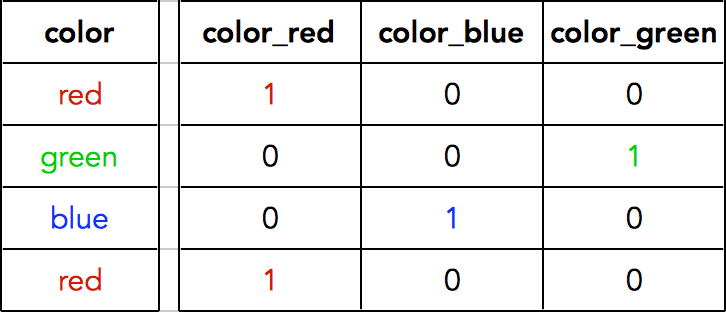
\includegraphics[width=0.6\textwidth]{Figures/one_hot_encoding}
	\caption{Ejemplo One hot encoding \\ Fuente:  \href{https://www.machinelearningplus.com/machine-learning/caret-package/attachment/one-hot-encoding/}{\textit{https://www.machinelearningplus.com/}}}
	\label{one}
\end{figure} 
En nuestra implementación fue necesario encontrar una representación para nuestras 10 clases de números. El código puede ser encontrado en el Apéndice \ref{onehot} .


\section{Modelo de la red neuronal}

En esta sección  veremos algunos modelos que fueron entrenados para la tarea de clasificación de audios de números estos serán probados con un solo tipo de redes RNN(ver \ref{redesrecurrentes}) y en especial su derivado LSTM(ver \ref{lstmlabel}).
\subsection{RNN}
Definimos un red neuronal con una sola capa RNN y una capa densamente conectada( ver Figura \ref{RNNNNN}). Esta red será probada con distintas cantidades de estados ocultos. Podemos ver el código de esta red en \ref{RNNCODE}



\subsection{LSTM}
Las redes LSTM son tipo de redes recurrentes especial que resuelven las dificultades de las RNN simples.
Dentro de las redes LSTM usaremos el esquema sin Dropout(\ref{LSTMESQUEMA}) y con Dropout(\ref{LSTMESQUEMA1DROP}). Los códigos de estos modelos son encontrados en los códigos \ref{LSTMCODE} y \ref{LSTMCODEDROP}.


\subsection{2 capas LSTM y 2 Dropout}
Adicionalmente se diseño una red con más de 2 capas LSTM para realizar las tareas de reconocimiento de voz. El esquema de esta red puede ser encontrado en \ref{2LSTMESQUEMA} y la implementación puede ser visto en el código \ref{2LSTM2DROPCODE} del Apéndice.

\subsubsection{Categorical Crossentropy}

Para entrenamiento de nuestro modelos usaremos categorical crossentropy como nuestra función de perdida.
	\begin{equation}
\label{CCE}
\begin{aligned}
CCE=-\frac{1}{N}\sum_{i=0}^{N}\sum_{j=0}^{J} y_{j}\log(\hat{y_{j}})+(1-y_{j})\log(1-\hat{y_{j}})
\end{aligned}
\end{equation}
\begin{itemize}
	\item N: cantidad del conjunto training
	\item J: cantidad de clases
\end{itemize}

\subsubsection{Adam}
Como algoritmo de optimización utilizaremos Adam, calcula una tasa de aprendizaje adaptativo para cada parámetro y es usado para optimizar la gradiente de descenso.
En la ecuación 5.2 mostramos el cálculo del promedio de decaimiento de las gradientes pasadas $m_{t}$ y el cuadrado de las gradientes pasadas $v_{t}$
\begin{equation}
\label{adam1}
\begin{aligned}
m_{t} &= \beta_{1} m_{t-1} +(1-\beta_{1})g_{t} \\
v_{t} &= \beta_{2} v_{t-1} +(1-\beta_{2})g_{t}^2
\end{aligned}
\end{equation}

\begin{itemize}
	\item $m_{t}:$ Primer momento (media)
	\item $v_{t}:$ Segundo momento de la gradiente
	\item $\beta_{1}:$ Taza de decaimiento del primer momento.
	\item $\beta_{2}:$ Taza de decaimiento del segundo momento.
\end{itemize}
En la ecuación 5.3 mostramos la forma de calcular estimado de la primer y segundo momento.
\begin{equation}
\label{adam2}
\begin{aligned}
\hat{m_{t}}&= \frac{m_{t}}{1-\beta_{1}^{t}} \\
\hat{v_{t}} &= \frac{v_{t}}{1-\beta_{2}^{t}}
\end{aligned}
\end{equation}

\begin{itemize}
	\item $\hat{m_{t}}:$ Estimación del Primer momento (media)
	\item $\hat{v_{t}}:$ Estimación del Segundo momento de la gradiente.
\end{itemize}

La ecuación 5.4 muestra la regla de actualización en Adam. Se utiliza el $\epsilon$ para prevenir una división por cero.
\begin{equation}
\label{adam3}
\begin{aligned}
\theta_{t+1}&= \theta_{t+1} - \frac{\eta}{\sqrt{\hat{v_{t}}}+\epsilon} \hat{m_{t}}	
\end{aligned}
\end{equation}

En el código 5.7 mostramos el uso del función de perdida y el optimizador como parte de la configuración de nuestro modelo.
